\documentclass[../../General.tex]{subfiles}
\begin{document}

\section{Diagrama de flujo general}


En la Figura \ref{fig:DiagramaFlujoGeneral}, se detalla la secuencia lógica de arranque y la arquitectura multitarea que gobierna la computadora principal del robot. El proceso inicia con la energización del hardware, donde el sistema operativo inicializa los buses de comunicación y declara una variable global de estado o Flag de Alerta en valor nulo. Posteriormente, el equipo entra en un estado de espera hasta recibir el comando inalámbrico de inicio por parte del operario.

Una vez activado, el software ejecuta una bifurcación propia de arquitecturas orientadas a eventos, dividiendo el procesamiento en hilos paralelos que operan de forma concurrente: un hilo de navegación, un hilo de telemetría y un hilo supervisor de seguridad. En lugar de que cada subproceso gestione sus propias condiciones de parada, los hilos paralelos operan exclusivamente como publicadores de estado. Simultáneamente, el hilo supervisor evalúa la Flag de Alerta de forma continua; si detecta un cambio de estado a valor activo, el supervisor ejecuta una interrupción de máxima prioridad que anula la tracción y transita al sistema hacia un modo seguro.

\begin{figure}[H]
	\captionsetup{justification=raggedright, singlelinecheck=false, labelsep=none}
	
	\caption[Diagrama de flujo de proceso general.]{} 
	
	\textit{Diagrama de flujo de proceso general.} \par\medskip
	
	\centering
	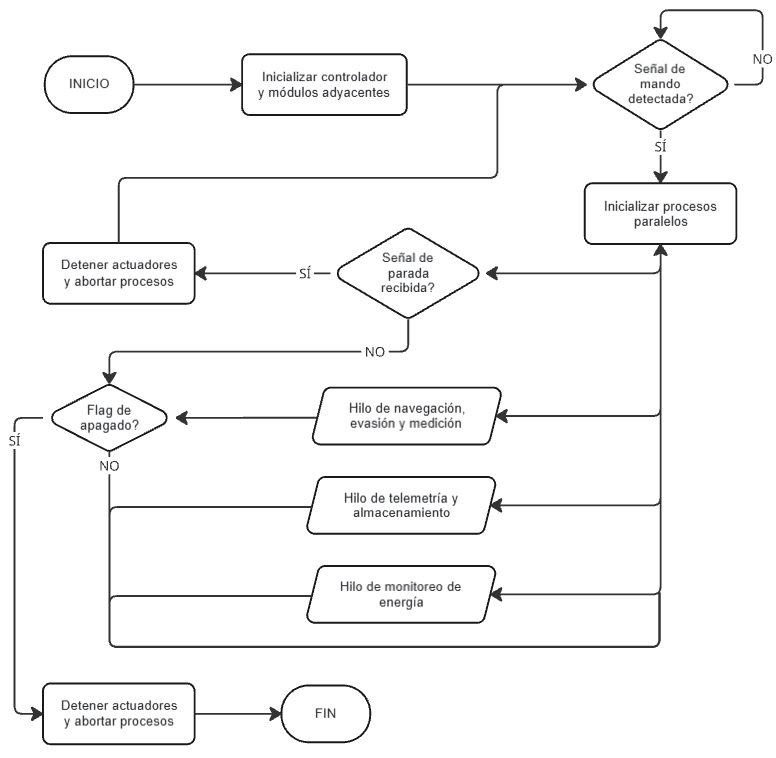
\includegraphics[width=\textwidth]{Recursos/Imagenes/ImagenesDisenoProgramacion/FlujoPrincipal.png} \par\medskip
	
	\raggedright
	\footnotesize \textit{Nota.} Elaboración propia.
	\label{fig:DiagramaFlujoGeneral}
\end{figure}


\end{document}